section{Comparison of NLP Models}
\label{sxn:nlp}

In this section, we examine quality metrics described in Section~\ref{sxn:methods} for several NLP model architectures.
%
%In particular, 
Within the past two years, nearly 100 open source, pre-trained NLP DNNs based on the revolutionary Transformer architecture have emerged.
These include variants of BERT, Transformer-XML, GPT, etc.
%
The Transformer architectures consist of blocks of so-called Attention layers, containing two large, Feed Forward (Linear) weight matrics~\cite{Attn2017}. 
In contrast to smaller pre-Activation maps arising in Cond2D layers, Attention matrices are significantly larger.
In general, we have found that they have larger $\alpha$ PL exponents.
Based on HT-SR Theory, 
%(in particular, the interpretation of values of $\alpha \sim 2$ as modeling systems with good correations over many size scales~\cite{BouchaudPotters03, SornetteBook}), 
this suggests that these models fail to successfully capture many of the correlations in the data (relative to their size) and thus are substantially \emph{under}-trained.
%
More generally, compared to the CV models of Section~\ref{sxn:cv},
modern NLP models have larger weight matrices and display different spectral properties, and 
%, both in terms of their architecture (e.g., wheter there are convolutions) as well as how they are used (e.g., whether one uses prediction error or perplexity).
thus, they provide a very different test for our empirical quality metrics.

Where Norm-base metrics perform reasonably well on well-trained NLP models, they behave anomalously poorly-trained models.
Indeed, in ``bad models'', the weight matrics may display rank collapse, decreased Frobeinus mass, or unsually small Spectral norms, 
which may be mis-interpreted as ``smaller is better.''
In contast, PL-based metrics (the log $\alpha$-Norm metric, 
$(\log\Vert\mathbf{W}\Vert_{\alpha}^{\alpha})$, and the Weighted Alpha metric, $\hat\alpha =\alpha\log\lambda_{max} $) display consistant behavior even on poorly trained models, and we can use these metrics to help indentify
where the archiectures need repair, and/or more and/or better data is needed.

%We now look in detail at the alpha metric, the spectral norm, and the new norm.
%We compare good and bad models, and a series of increasingly big models
%trained on big data sets.  We show why alpha works but spectral norm is not enough.
%The layer Spectral Norm behaves unexpectedly, while $\alpha$-based metrics can give insight into how well trained a model is.

%\michael{WHERE: Say large $\alpha$ values don't mean much.}
\paragraph{What does large $\alpha$ mean?}
We do note, however, that many NLP models, such as the GPT and BERT, may have weight matrices with unusually large PL exponents
($\alpha\gg 6$), which indicates these matrices may be \emph{under}-correlated (i.e over-parameterized), although the truncated PL fit
itself may not be very reliable because the MLE estimator is unreliable in this range.  Phenomenologically, if we examine
the ESD visually, we can usually describe these $\mathbf{W}$ as in the \emph{Bulk-Decay} or \emph{Bulk-plus-Spikes} phase\cite{MM}.
We have conjectured previously that very well-trained DNNs would not have many \emph{outlier} $\alpha>6$, 
and improved versions of GPT (shown below, and BERT (not shown) confirm this.

%\michael{WHERE: Highlight difference between $\alpha$ and $\hat{\alpha}$.}
\paragraph{The differences between $\alpha$ and $\hat{\alpha}$.}
To avoid confusion, let us clarify the differences between $\alpha$ and $\hat{\alpha}$.  
We fit the ESD of the correlation matrix $\mathbf{X}$ to a truncated power law (PL), parameterized by 2 values:
the PL exponent $\alpha$, and the maximum eigenvalue $\lambda_{max}$.  (Technically, we also need the minimum
eigenvalue $\lambda_{min}$, but this detail does not affect our analysis.)
The PL exponent $\alpha$ measures of the 
amount of correlation in a DNN layer weight matrix $\mathbf{W}$.  It is valid for $\lambda<\lambda_{max}$, and
it scale invariant (does not depend on the normalization of $\mathbf{W}$ or $\mathbf{X}$.)
The Weighted-Alpha metric, $\hat{\alpha}=\alpha\log\lambda_{max}$, approximates the log $\alpha$ Norm.
$(\log\Vert\mathbf{X}\Vert^{\alpha}_{\alpha})$ (derived using statistical mechanics and RMT \nred{(in progress)}, 
and lets us compute a balanced, weighted average log PL norm metrix for the entire DNN.  
The $\hat{\alpha}$ metric also behaves like an imrpoved, weighted log average Spectral Norm, and may track this metric in some cases.

\paragraph{OpenAI GPT Models.}

The OpenAI GPT and GPT2 models provide us with the opportunity to analyze two effects: training the same model with different data set sizes; and increasing sizes of both the data set and architectures.
These models have the remarkable ability to generate fake text that appears to the human to be real, and they have generated significant media attention because of the potential for their misuse.
For this reason, the original GPT model released by OpenAI was trained on on a deficient data set, rendering the model interesting but not fully functional.  
Later, OpenAI released a much improved model, GPT2 (small), which has the same architecture and number of layers as GPT, but which has been trained on a larger and better data set (and with other changes), making it remarkably good at generating (near) human-quality fake text.  
%
By comparing the poorly-trained GPT to the well-trained GPT2, we can indentify empirical indidcators for when a model has in fact been poorly-trained and thus may perform poorly when deployed.

\charles{More details here.}
The GPT models we analyze are deployed with the popular HuggingFace PyTorch library~\cite{XXX-XXX}.
GPT has 12 layers, with 4 Multi-head Attention Blocks, giving $48$ layer Weight Matrices $\mathbf{W}$.
Each Block has 2 components, the Self Attention (attn) and the Projection (proj) matrics.  
The self-attention  matrices are larger, of dimension ($2304\times 768$) or ($3072\times 768$).
The projection layer concatenates the self-attention results into a vector (of dimension $768$).
This gives $50$ large matrices.
%
Because GPTand GPT2 are trained on different data sets, the initial Embedding matrices differ in shape.
GPT has an initial Token and Positional Embedding layers, of dimension $(40478\times 768)$ and $(512\times 768)$, respectively, whereas GPT2 has input Embeddings of shape $(50257\times 768)$ and $(1024\times 768)$, respectively. 
%
The OpenAI GPT2 (English) models are: \nred{GPT2-small, GPT2-medium, GPT2-large, and GPT2-xl}, \
having include $12, 24, 36, \text{and }48$ layers, respectively, with increasingly larger weight matrices.
%The model card for GPT2 is published on github.\footnote{\url{https://github.com/openai/gpt-2/blob/master/model_card.md}}.


\begin{table}[t]
\small
\begin{center}
%\begin{tabular}{|p{1in}|c|c|c|c|c|}
\begin{tabular}{|p{0.75in}|c|c|c|c|c|}
\hline
 Series  & \#   & $\langle\log\Vert\mathbf{W}\Vert_{F}\rangle$ & $\langle\log\Vert\mathbf{W}\Vert_{\infty}\rangle$ & $\hat{\alpha}$ & $\langle\log\Vert\mathbf{X}\Vert^{\alpha}_{\alpha}\rangle$ \\
\hline
GPT & 49 & 1.64  & 1.72 & 7.01 & 7.28 \\
GPT2-small & 49 & 2.04  & 2.54& 9.62 & 9.87 \\
\hline
GPT2 medium & 98 & 2.08 & 2.58& 9.74 & 10.01 \\
GPT2 large & 146 & 1.85 & 1.99& 7.67 & 7.94 \\
GPT2 xl & 194 & 1.86 & 1.92 & 7.17 & 7.51 \\
\hline
\end{tabular}
\end{center}
\caption{Average value for the Average log Norm metrics and the Weighted Alpha metric for pretrainnd OpenAI GPT and GPT2 models. Column \# refers to number of layers treated.  Note averages do not include the first embedding layer(s) because they are not (implicitly) normalized.  }
\label{table:nlp}
\end{table}


\paragraph{Coarse Analysis: Empirical Quality Metrics for GPT and GPT2.}

We have analyzed the four quality metrics described in Section~\ref{sxn:methods} for the OpenAI GPT and GPT2 pretrained models.
See Table \ref{table:nlp} for a summary of results.
We start by examining the PL exponents $\alpha$ for GPT and GPT2-small.
Observe that all four metrics increase when going from GPT to GPT2-small, i.e., they are smaller for the higher-quality model (higher quality since GPT was trained to better data), when the number of layers is held fixed.
Observe also that (with one minor exception involving the log Frobenius norm metric) all four metrics decrease as one goes from GPT2 medium to large to xl, indicating that the larger models indeed look better than the smaller models.
%(The one minor exception is the log Frobenius norm increasing from $1.85$ to $1.86$, for GPT2 large to GPT2 xl.)

Figure~\ref{fig:GPT-alpha-hist} shows the histogram (empirical density), for all layers, of $\alpha$ for GPT (blue) and this GPT2 (red) model.  
These two histograms are very different, with GPT2 having both a notably smaller mean $\alpha$, and far fewer unusually-large outlying $\alpha$ values.

From this, we see that $\alpha$ provides a good quality metric for comparing these two models, the``bad'' GPT vs. the ``good'' GPT2.
The deficient GPT has numerous unsually large $\alpha$ exponents--meaning they are not Heavy Tailed at all.
Indeed, we expect that a poorly trained model lack Heavy Tailed behavior in all layers.
On the other hand, as expected, the improved GPT2 model has, on average, smaller $\alpha$ than the older GPT, with all $\alpha\le6$.  


\paragraph{Scale Collapse in Poorly Trained Models}
However, as seen in Figure \ref{fig:GPT-snorm-hist},
the ``bad'' GPT model has, spuriously, many smaller Spectral Norms $(\log\Vert\mathbf{W}\Vert_{\infty})$,
compared to the ``good'' GPT2--which violates the belief that smaller Spectral Norms are always better.
Indeed, because there are so many anonymously small $\Vert\mathbf{W}\Vert_{\infty}$,
it appears that the GPT model may be exhibiting the \emph{scale collapse} observed
in the distilled CV models (above).
This is an extremely important observation because it demonstrates that while the Spectral Norm
may correlate well with predicted test error, it is not a good indicator of the overall quality of a model,
and using it as an empirical metric may give spurious results when applied to poorly trained
or otherwise deficient models. 

\begin{figure}[h]
    \centering
    \subfigure[Power law exponent ($\alpha$)]{
        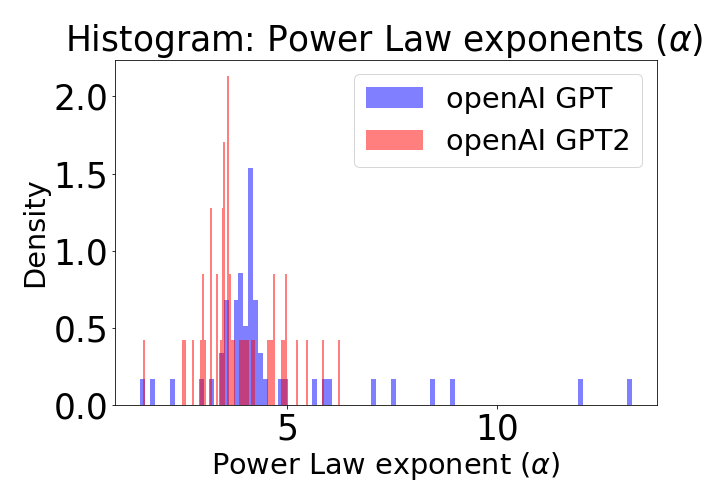
\includegraphics[width=4.0cm]{img/GPT-alpha-hist.png}
        \label{fig:GPT-alpha-hist}
       }
    %\qquad
    \subfigure[Spectral Norm $(\log\Vert\mathbf{W}\Vert_{\infty})$]{
        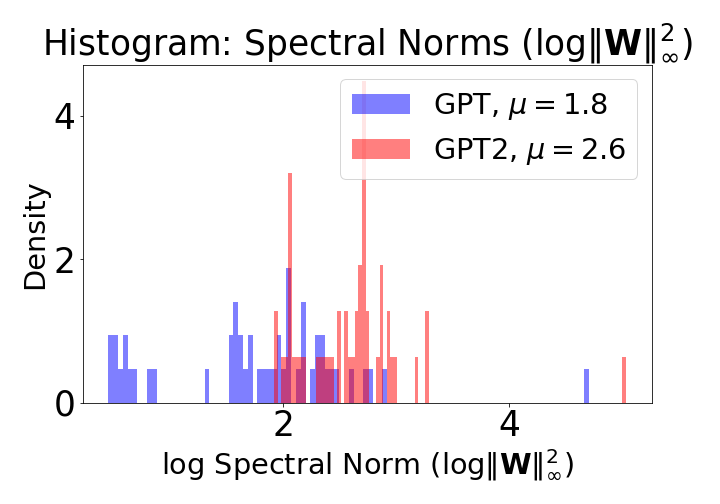
\includegraphics[width=4.0cm]{img/GPT-snorm-hist.png}
        \label{fig:GPT-snorm-hist}
       }
   \caption{Comparison of PL exponents, $\alpha$, and log Spectral Norms, 
$(\log\Vert\mathbf{W}\Vert_{\infty})$, for the OpenAI GPT and GPT2 (small) pretrained models.}
   
\label{fig:GPT-hist}
\end{figure}





Note that Figure \ref{fig:GPT-snorm-hist} also shows some unusually large Spectral Norms, but,
here, simply correspond to the change in normalization of the word embedding layer(s) and can be ignored.
From Figure \ref{fig:gpt-snorm-layer} (below), we see that these correspond to the first embedding layer(s).
These layers appear to have a different effective normalization, and therefore a different scale.
\charles{We discuss this further in the Appendix}
%For example, in GPT, most layers, the maximum eigenvalue $\lambda_{max}\sim\mathcal{O}(10-100)$,
%but in the first embedding layer, the maximum is of order N (the number of words in the embedding), or
% $\lambda_{max}\sim\mathcal{O}(10^{5})$.  For GPT and GPT2, we treat all layers as-is (although one may to normalize
%the first 2 layers by  $\mathbf{X}$ by $\frac{1}{N}$, or to treat them as an outlier).
Here, we do not include them in our computed average metrics in Table \ref{table:nlp},
and do not include them in the histogram plot in Figure \ref{fig:GPT-snorm-hist}.

\paragraph{Layer Analysis: Correlation Flow in GPT and GPT2.} 

also differs significantly between GPT and GPT2.
Figure \ref{fig:gpt-alpha-layer} plots $\alpha$ vs the depth (i.e. a layer id) for each model.
The deficient GPT model displays two trends in $\alpha$ , one stable with $\alpha\sim 4$,
and one increasing with layer id, with $\alpha$ reaching as high as $12$.
In contrast, the well-trained GPT2 model shows consistant and stable patterns, again
with one stable $\alpha\sim 3.5$ (and below the GPT trend), and the other only
slightly trending up, with $alpha\le 6$. 
The scale-invariant $\alpha$ metric lets us identify potentially
poorly-trained models.

Notice also that the Spectral Norms
(Figure \ref{fig:gpt-snorm-layer})
and the $\alpha-$Norms
(Figure \ref{fig:gpt-pnorm-layer})
display an unusually some mall values for GPT,
and some increasing trending values for GPT2.
Generally speaking, we do not think scale-dependennt 
norm metrics can be directly applied to distinguish ``good'' vs ``bad'' models 
because of the anamalous scale collapse that is frequently observed in bad models.

\begin{figure}[htb]
    \centering
    \subfigure[Power Law exponent $(\alpha)$]{
        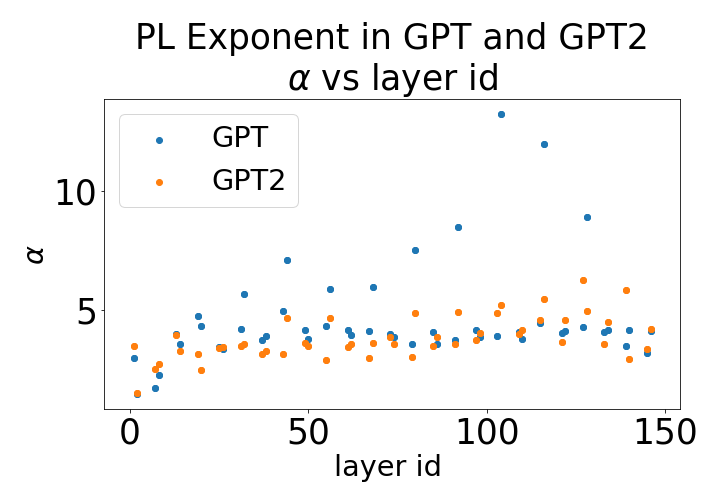
\includegraphics[width=4.0cm]{img/GPT-alpha-depth.png}
        \label{fig:gpt-alpha-layer}
    }
    \subfigure[Spectral Norm $(\log\Vert\mathbf{W}\Vert_{\infty})$]{
        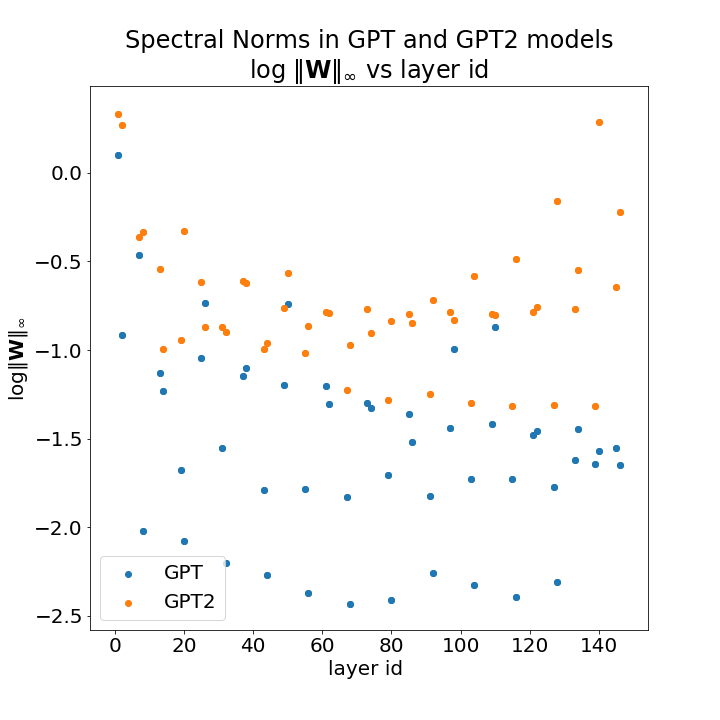
\includegraphics[width=4.0cm]{img/GPT-snorm-depth.png}
        \label{fig:gpt-snorm-layer}
    }
    \caption{Comparison of Correlation Flow and Spectral Norm for OpenAI GPT and GPT2   }
    \label{fig:gpt-alpha-layers}
\end{figure}


\paragraph{GPT2: medium, large, xl} 
We now look across the series of increasingly improving GPT2 models, (i.e. ``good, better, best''), 
by examining both the PL exponent $\alpha$, as well as the various log Norm metrics.  
In general, as we move from GPT2-small to GPT2-xl, 
the histograms for both $\alpha$ exponents and the log Norm metrics downshift from larger to smaller values. 
See Figure \ref{fig:gpt2-histograms}, which shows the histograms over the layer weight matrics
for fitted $\alpha$, and the log Spectral Norm
 $(\log\Vert\mathbf{W}\Vert_{\infty})$  
and log Alpha Norm
 $(\log\Vert\mathbf{W}\Vert_{\alpha}^{\alpha})$ 
metrics.

We see that the average $\alpha$ decreases with increasing model size, although the differences are less noticible 
between the differing ``good, better, best'' GTP2 models than between the ``good vs bad'' GPT2 and GPT models.
Unlike GPT, however, the layer (log) Spectral Norms $(\log\vert\mathbf{W}\Vert_{\infty})$ 
and (log) Alpha Norms $(\log\vert\mathbf{W}\Vert_{\alpha}^{\alpha})$
behave more as expected for GPT2 layers, with the larger models, consistently having smaller norms. 
Likewise, Figure \ref{fig:gpt2-snorm-hist} shows decreasing average log Spectral Norms with the larger models.  
As expected, the norm metrics can indeed distinguish among ``good, better, best'' models
among a series well trained models.

We do notice, however, that while the peaks of the $\alpha$ is getting smaller, 
towards $2.0$,
the tails of the distribution shifts right, with larger GPT2 models having more
usually large $\alpha$.  
We suspect this indicates that these larger GPT2 models are over-parameterized/under-optimized and 
that they have capacity to support datasets even larger than the recent XL $1.5B$ release~\cite{gpt2-xl}.

\begin{figure}[htb]
    \centering

    \subfigure[PL exponent ($\alpha$)]{
        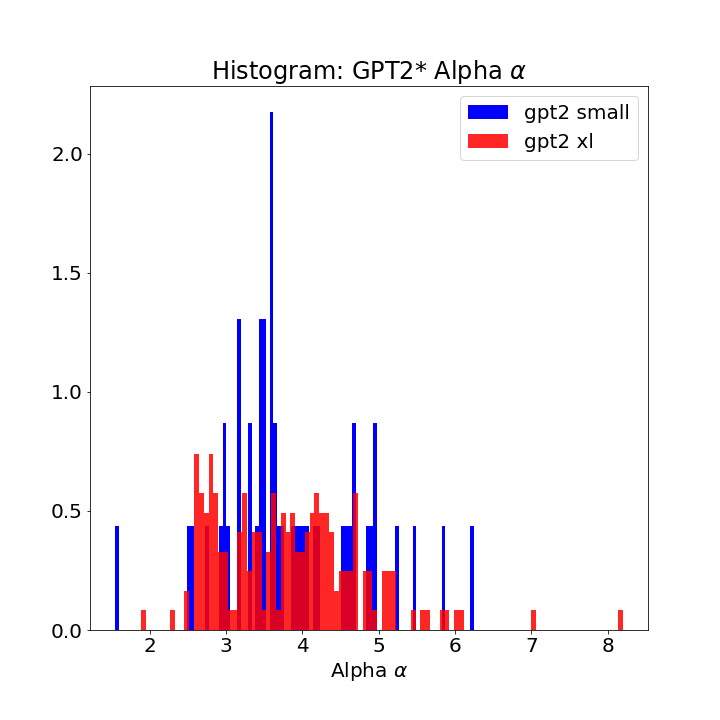
\includegraphics[width=4.0cm]{img/GPT2*_fnl_alpha_hist.png}
        \label{fig:gpt2-alpha-hist}
    }
    \subfigure[log Alpha Norm]{
        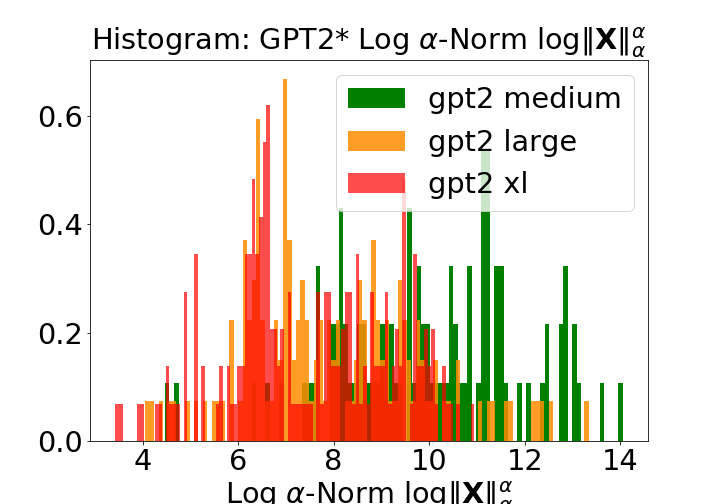
\includegraphics[width=4.0cm]{img/GPT2*_fnl_logpnorm_hist.png}
        \label{fig:gpt2-pnorm-hist}
    }
    \caption{PL exponents ($\alpha$), log Spectral norm $(\log\Vert\mathbf{W}\Vert_{\infty})$, and log Alpha norm $(\log\Vert\mathbf{X}\Vert_{\alpha}^{\alpha})$ for different size models in the GPT2 architecture series.  (Plots omit the first 2 (embedding) layers, because they are normalized differently giving anamolously large values.)}
    \label{fig:gpt2-histograms}
\end{figure}
